\lab{Applications}{Riemann Sphere and Mobius Transformations}{Riemann Sphere and Mobius Transformations}

\objective{Understand the Riemann Sphere in graphics applications.}

We have now examined several applications of complex numbers and functions.
In this lab we extend several of these ideas and develop some intuition about the Riemann sphere using visualization techniques in Python.

Recall that the complex numbers are an extension of the real numbers that include the imaginary numbers.
We extend them even further in this section and examine the extended complex numbers.
Similar to the extended real numbers, the extended complex numbers are our regular set of complex numbers with the addition of a point at infinity.
This allows us to examine, for example, certain quotients that are undefined on the standard complex numbers.

The Riemann sphere construction allows a compact and intuitive construction of the extended complex numbers.
Consider the standard complex plane, only now in 3-space instead of a 2 dimensional plane.
Let the $x$-axis correspond to the real part of the complex numbers and let the $y$-axis correspond to the imaginary part.
Let $z=0$ for all $x$ and $y$. 

Now consider a the unit sphere centered at $(0,0,1)$ combined with the complex numbers in 3-space.
We may map every point of the extended complex plane onto this sphere.
Let infinity correspond to the point $(0,0,2)$ at the very top of the sphere.
For all other points on the complex plane consider the line between the point on the complex plane and the point at the top of the sphere.
Let each point of the complex plane map to the point where this line intersects with the surface of the sphere.
Note that for any complex number, there is exactly one such point.
This construction is illustrated in Figure \ref{riemann:stereographic}

\begin{figure}
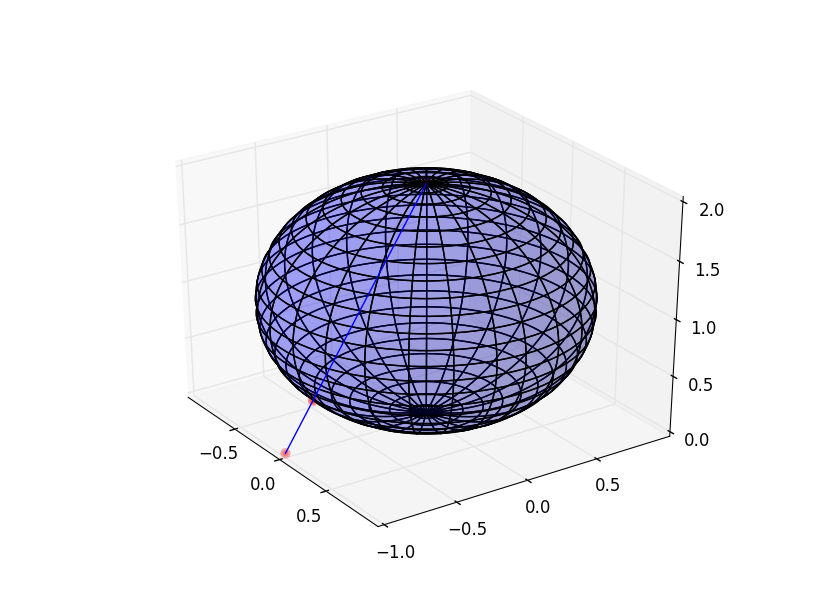
\includegraphics[width=\textwidth]{StereographicIllustration.png}
\caption{Stereographic projection of a point in the complex plane onto the unit sphere.}
\label{riemann:stereographic}
\end{figure}

\begin{problem}  Write a function that, given a complex number, returns the coordinates of the corresponding point on the riemann sphere in 3-space.
\end{problem}

\begin{problem}
Write a function that, given the coordinates of a point on the Riemann Sphere, returns the corresponding point on the complex plane.
If the input point is $(0,0,2)$ have your function return "infinity."
\end{problem}

\section*{Mobius Transformations}

Recall from the previous chapter that a conformal mapping is a complex function that preserves angles between lines.
We now examine a special kind of conformal mapping called a Mobius transformation (not to be confused with the Mobius Transform), or a fractional linear transformation.
We first give the definition of a fractional linear transformation, and then examine what sorts of transformations we can do with them.

\begin{definition} A fractional linear transformation is a any complex function of the form
\[
f(z) = \frac{az + b}{cz + d}
\]
 Where a, b, c, and d are complex numbers with the restriction that $ad \neq bc$.
\end{definition}

Fractional linear transformations are versatile enough to include translations, rotations, magnifications, or any combination of the same, of shapes in the complex plane.
For example, if we wish to magnify the unit disk by a factor of 2 and then translate it up 2 along the imaginary axis, we would use the following transformation:
\[
f(z)=2z+2i
\]

\begin{figure}
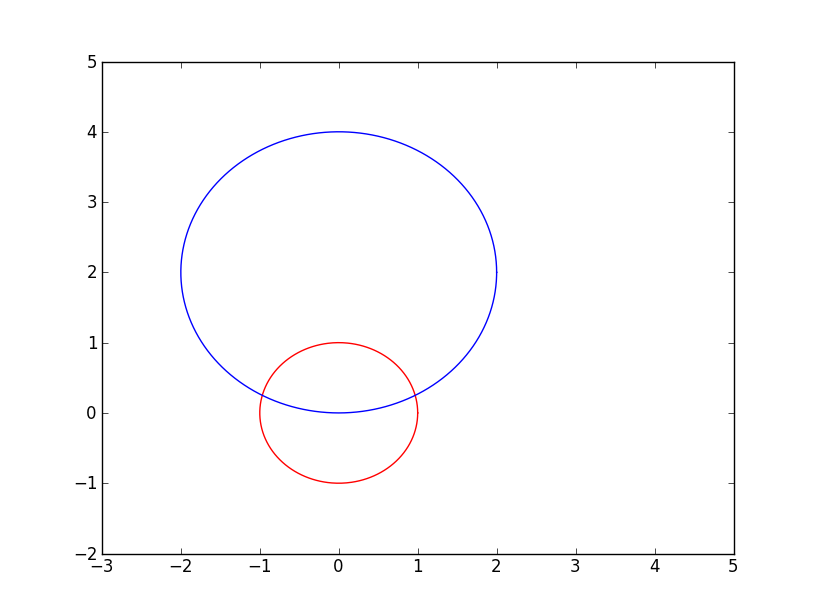
\includegraphics[width=\textwidth]{mobius1.png}
\caption{The unit disk and its image under the transformation $2z+2i$.}
\label{riemann:mobius1}
\end{figure}

\begin{problem} Write a Python function that accepts arguments $a,b,c,$ and $d$.
Perform the corresponding fractional linear transformation on a grid inside the box $[-1,1]\times[-i,i]$, and then visualize the box before and after the transformation on the same plot, but using different colors.
\end{problem}

We now will mention some of the important properties of fractional linear transformations.

With some manipulation, it can be shown that:

$$\frac{az+b}{cz+d}=\frac{a}{c}+\frac{bc-ad}{c} \frac{1}{cz+d}$$

This implies that any fractional linear transformation can be represented as the composition of the functions $\alpha x$, $x+\beta$, and $\frac{1}{x}$ where $\alpha$ and $\beta$ are complex. 

This allows us to determine some things about the properties of fractional linear transformations.
Since each of those functions is holomorphic wherever it is defined, we may say the same of their composition.
In other words, our fractional linear transformation is holomorphic except at $z=-\frac{d}{c}$, or if $c=0$, the transformation is holomorphic at all points in the complex plane. 

Since fractional linear transformations are holomorphic, they are also conformal.
This can also be readily derived by considering a fractional linear transformation as the composition of the functions above.
If each of the functions above is conformal on a domain, their composition will also be conformal on that domain. 

We will now consider the effects of fractional linear transformations on points of the Riemann Sphere.
Figures \ref{riemann:mobius2} and \ref{riemann:mobius3} show a grid on the complex plane, it's projection onto the Riemann Sphere, the image of the grid under the transformation $\frac{1}{z}$, and it's projection onto the Riemann Sphere. 

\begin{figure}
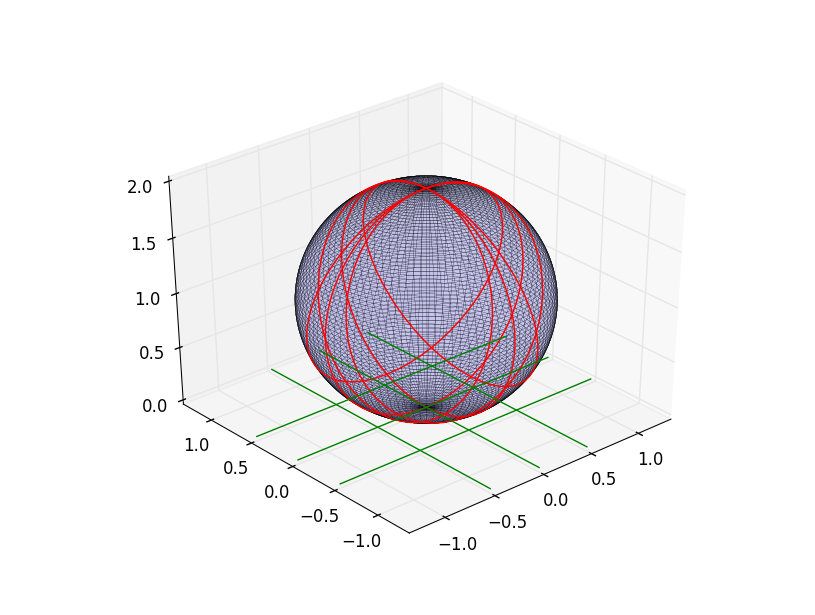
\includegraphics[width=\textwidth]{mobius2.png}
\caption{The Riemann Sphere witha $3\times 3$ grid projected onto it.}
\label{riemann:mobius2}
\end{figure}

\begin{figure}
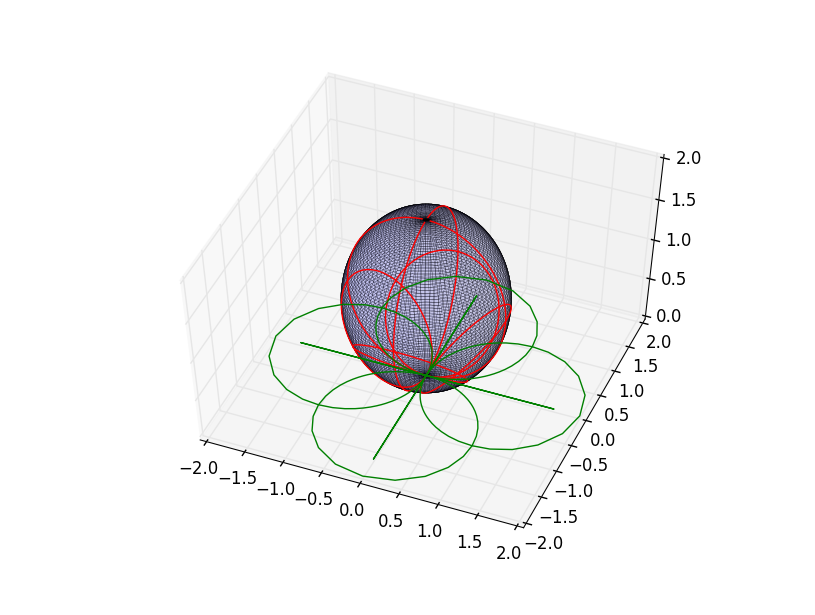
\includegraphics[width=\textwidth]{mobius3.png}
\caption{The images of the Riemann Sphere and the $3\times 3$ grid shown in Figure \ref{riemann:mobius2} under the transformation $\frac{1}{z}$.}
\label{riemann:mobius3}
\end{figure}

Notice how both circles and lines on the complex plane are circles on the Riemann Sphere.
A line on the complex plane is really just a circle on the Riemann Sphere that passes through the point at infinity.
An interesting property of fractional linear transformations is that they are circle preserving.
This means that the image of a circle on the Riemann Sphere under any fractional linear transformation is also a circle on the Riemann Sphere.
In terms of the standard complex plane, we may say that the image of any circle or line is a circle or line.

This can be proven analytically by considering the equation of a circle on the complex plane.
Let $z=a=bi$.
For some circle centered at a point $E=\alpha + \beta i$ with radius $r$, $a$ and $b$ will satisfy the equation $(a-\alpha)^2+(b-\beta)^2=r^2$.
Expanding this expression and simplifying we have:
$$a^2-b^2-2a\alpha-2b\beta+\alpha^2+\beta^2-r^2=0$$
Letting $D=\alpha^2+\beta^2-r^2$, we may rewrite the above equation as follows:
$$z\bar{z}+E\bar{z}+\bar{E}z+D=0$$
This gives motivation for the general equation of a circle in the complex plane.
$$Az\bar{z}+E\bar{z}+\bar{E}z+D=0$$
Where $A$ and $D$ are real and $E$ is complex.
If $A\neq 0$ and $E\bar{E}-AD>0$ then this is the equation of a circle.
Note that if $A=1$, $E$ is the center of the circle.
If $A=0$ then this is the equation of a line (or a circle through infinity on the Riemann Sphere).

Now to see that a fractional linear transformation is circle preserving, recall that it can be represented as the composition of the functions $\alpha x$, $x+\beta$, and $\frac{1}{x}$ where $\alpha$ and $\beta$ are complex.
If each of these functions is circle preserving, their composition will also be circle preserving, and we will have the desired result. 

The function $x+\beta$ is a translation and will clearly be circle preserving.

Letting $z=\alpha w$, we have: 
$$A\alpha \bar{\alpha} w\bar{w}+\bar{E}\alpha z+E\bar{\alpha} \bar{z}+D=0$$
which may be rewritten as:
$$A|\alpha|^2 w\bar{w}+\bar{(E\bar{\alpha})}z+E\bar{\alpha} \bar{z}+D=0$$
which is still the equation of a circle, so the function $\alpha z$ is also circle preserving.

Now, letting $z=\frac{1}{w}$, we have:
$$\frac{A}{w\bar{w}}+\frac{\bar{E}}{w}+\frac{E}{\bar{w}}+D=0$$
which we may rewrite as:
$$Dw\bar{w}+\bar{E}\bar{w}+Ew+A=0$$
which is, again, the equation of a circle.

Since each of these functions is circle preserving, any composition of these functions will also be circle preserving, so all fractional linear transformations are circle preserving.

\begin{problem}
Write a python function which accepts the constants $a$, $b$, $c$, and $d$ and returns the constants $A$, $E$, and $D$ of the general equation of the image of the unit circle ($A = 1$ and $D = -1$) under the corresponding fractional linear transformation. Just replace $z$ and $\bar{z}$ with $f(z)$ and $f(\bar{z})$, multiply out the denominators, and group like terms of $z$ to find the new $A$,$E$, and $D$ in terms of $a$, $b$,$c$, and $d$.
\end{problem}

Fractional linear transformations have varied effects on the Riemann Sphere.
A simple example is the transformation $e^{\frac{\pi i}{4}}z$ which rotates the entire complex plane 45 degrees.
This transformation is shown in Figure \ref{riemann:mobius4}.

\begin{figure}
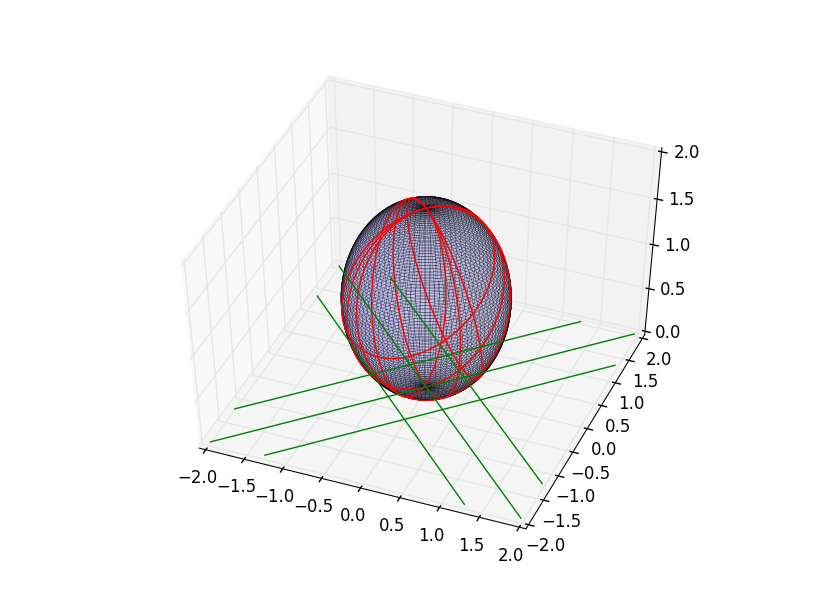
\includegraphics[width=\textwidth]{mobius4.png}
\caption{The images of the Riemann Sphere and the $3\times 3$ grid shown in Figure \ref{riemann:mobius2} under the transformation $e^{\frac{\pi i}{4}}z$.}
\label{riemann:mobius4}
\end{figure}

We can also rotate the Riemann Sphere in other directions.
The transformation $\frac{2z+4}{-iz+2i}$ rotates the Riemann sphere 90 degrees in the x-z plane.
Figure \ref{riemann:mobius5} is a plot of the same grid under that transformation.

\begin{figure}
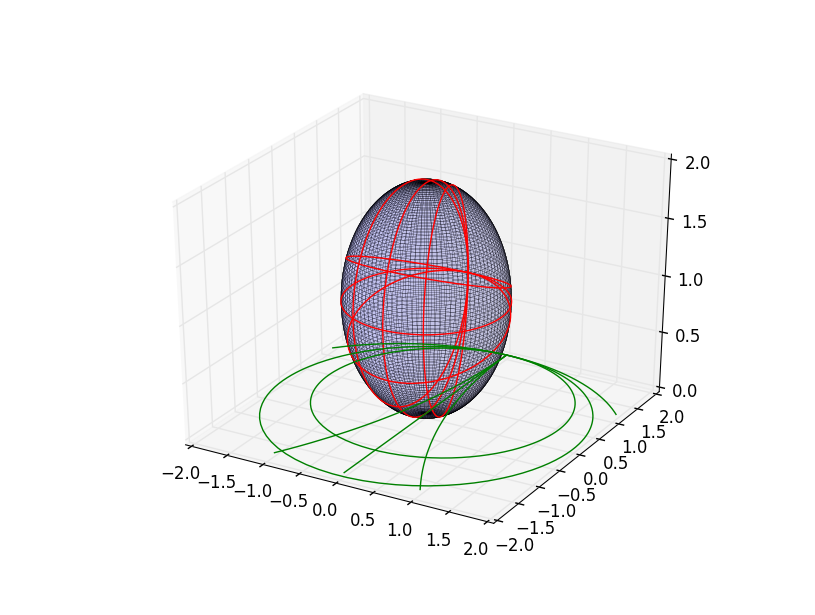
\includegraphics[width=\textwidth]{mobius5.png}
\caption{The images of the Riemann Sphere and the $3\times 3$ grid shown in Figure \ref{riemann:mobius2} under the transformation $\frac{2z+4}{-iz+2i}$.}
\label{riemann:mobius5}
\end{figure}

\begin{comment}
\begin{problem}#This proof is easy, but we're cutting out the proof problems
The matrix representation of the fracional linear transformation $\frac{az+b}{cz+d}$ is:
\[
\begin{pmatrix}
a&b\\
c&d
\end{pmatrix}
\]
Prove that for two fractional linear transformation $f$ and $g$ with matrix representations $F$ and $G$ that the matrix representation of $f(g(z))$ is $FG$.
\end{problem}
\end{comment}
As a note, it turns out that you can define a fractional linear transformation by specifying 3 points and their images under the transformation. In other words, since a circle can be defined on the complex plane by just three points, a fractional linear transformation can be defined by how it transforms a circle. However, the algebra is somewhat time consuming to find the transform from 3 points and their images and is best done with a symbolic solver.

\begin{comment}
%the algebra on this problem was a little too difficult
\begin{problem}
It turns out that we can define a fractional linear transformation by specifying 3 points and their images under the transformation.
Write a python function that accepts two lists of three complex numbers and returns the matrix representation of the fractional linear transformation that maps the numbers of the first list to the numbers of the second list.
\end{problem}
\end{comment}
